\documentclass[1p]{elsarticle_modified}
%\bibliographystyle{elsarticle-num}

%\usepackage[colorlinks]{hyperref}
%\usepackage{abbrmath_seonhwa} %\Abb, \Ascr, \Acal ,\Abf, \Afrak
\usepackage{amsfonts}
\usepackage{amssymb}
\usepackage{amsmath}
\usepackage{amsthm}
\usepackage{scalefnt}
\usepackage{amsbsy}
\usepackage{kotex}
\usepackage{caption}
\usepackage{subfig}
\usepackage{color}
\usepackage{graphicx}
\usepackage{xcolor} %% white, black, red, green, blue, cyan, magenta, yellow
\usepackage{float}
\usepackage{setspace}
\usepackage{hyperref}

\usepackage{tikz}
\usetikzlibrary{arrows}

\usepackage{multirow}
\usepackage{array} % fixed length table
\usepackage{hhline}

%%%%%%%%%%%%%%%%%%%%%
\makeatletter
\renewcommand*\env@matrix[1][\arraystretch]{%
	\edef\arraystretch{#1}%
	\hskip -\arraycolsep
	\let\@ifnextchar\new@ifnextchar
	\array{*\c@MaxMatrixCols c}}
\makeatother %https://tex.stackexchange.com/questions/14071/how-can-i-increase-the-line-spacing-in-a-matrix
%%%%%%%%%%%%%%%

\usepackage[normalem]{ulem}

\newcommand{\msout}[1]{\ifmmode\text{\sout{\ensuremath{#1}}}\else\sout{#1}\fi}
%SOURCE: \msout is \stkout macro in https://tex.stackexchange.com/questions/20609/strikeout-in-math-mode

\newcommand{\cancel}[1]{
	\ifmmode
	{\color{red}\msout{#1}}
	\else
	{\color{red}\sout{#1}}
	\fi
}

\newcommand{\add}[1]{
	{\color{blue}\uwave{#1}}
}

\newcommand{\replace}[2]{
	\ifmmode
	{\color{red}\msout{#1}}{\color{blue}\uwave{#2}}
	\else
	{\color{red}\sout{#1}}{\color{blue}\uwave{#2}}
	\fi
}

\newcommand{\Sol}{\mathcal{S}} %segment
\newcommand{\D}{D} %diagram
\newcommand{\A}{\mathcal{A}} %arc


%%%%%%%%%%%%%%%%%%%%%%%%%%%%%5 test

\def\sl{\operatorname{\textup{SL}}(2,\Cbb)}
\def\psl{\operatorname{\textup{PSL}}(2,\Cbb)}
\def\quan{\mkern 1mu \triangleright \mkern 1mu}

\theoremstyle{definition}
\newtheorem{thm}{Theorem}[section]
\newtheorem{prop}[thm]{Proposition}
\newtheorem{lem}[thm]{Lemma}
\newtheorem{ques}[thm]{Question}
\newtheorem{cor}[thm]{Corollary}
\newtheorem{defn}[thm]{Definition}
\newtheorem{exam}[thm]{Example}
\newtheorem{rmk}[thm]{Remark}
\newtheorem{alg}[thm]{Algorithm}

\newcommand{\I}{\sqrt{-1}}
\begin{document}

%\begin{frontmatter}
%
%\title{Boundary parabolic representations of knots up to 8 crossings}
%
%%% Group authors per affiliation:
%\author{Yunhi Cho} 
%\address{Department of Mathematics, University of Seoul, Seoul, Korea}
%\ead{yhcho@uos.ac.kr}
%
%
%\author{Seonhwa Kim} %\fnref{s_kim}}
%\address{Center for Geometry and Physics, Institute for Basic Science, Pohang, 37673, Korea}
%\ead{ryeona17@ibs.re.kr}
%
%\author{Hyuk Kim}
%\address{Department of Mathematical Sciences, Seoul National University, Seoul 08826, Korea}
%\ead{hyukkim@snu.ac.kr}
%
%\author{Seokbeom Yoon}
%\address{Department of Mathematical Sciences, Seoul National University, Seoul, 08826,  Korea}
%\ead{sbyoon15@snu.ac.kr}
%
%\begin{abstract}
%We find all boundary parabolic representation of knots up to 8 crossings.
%
%\end{abstract}
%\begin{keyword}
%    \MSC[2010] 57M25 
%\end{keyword}
%
%\end{frontmatter}

%\linenumbers
%\tableofcontents
%
\newcommand\colored[1]{\textcolor{white}{\rule[-0.35ex]{0.8em}{1.4ex}}\kern-0.8em\color{red} #1}%
%\newcommand\colored[1]{\textcolor{white}{ #1}\kern-2.17ex	\textcolor{white}{ #1}\kern-1.81ex	\textcolor{white}{ #1}\kern-2.15ex\color{red}#1	}

{\Large $\underline{12a_{0312}~(K12a_{0312})}$}

\setlength{\tabcolsep}{10pt}
\renewcommand{\arraystretch}{1.6}
\vspace{1cm}\begin{tabular}{m{100pt}>{\centering\arraybackslash}m{274pt}}
\multirow{5}{120pt}{
	\centering
	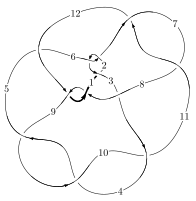
\includegraphics[width=112pt]{../../../GIT/diagram.site/Diagrams/png/1113_12a_0312.png}\\
\ \ \ A knot diagram\footnotemark}&
\allowdisplaybreaks
\textbf{Linearized knot diagam} \\
\cline{2-2}
 &
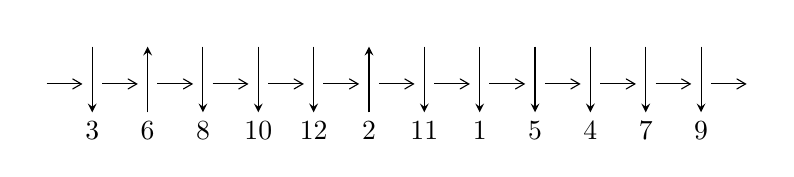
\begin{tikzpicture}[x=20pt, y=17pt]
	% nodes
	\node (C0) at (0, 0) {};
	\node (C1) at (1, 0) {};
	\node (C1U) at (1, +1) {};
	\node (C1D) at (1, -1) {3};

	\node (C2) at (2, 0) {};
	\node (C2U) at (2, +1) {};
	\node (C2D) at (2, -1) {6};

	\node (C3) at (3, 0) {};
	\node (C3U) at (3, +1) {};
	\node (C3D) at (3, -1) {8};

	\node (C4) at (4, 0) {};
	\node (C4U) at (4, +1) {};
	\node (C4D) at (4, -1) {10};

	\node (C5) at (5, 0) {};
	\node (C5U) at (5, +1) {};
	\node (C5D) at (5, -1) {12};

	\node (C6) at (6, 0) {};
	\node (C6U) at (6, +1) {};
	\node (C6D) at (6, -1) {2};

	\node (C7) at (7, 0) {};
	\node (C7U) at (7, +1) {};
	\node (C7D) at (7, -1) {11};

	\node (C8) at (8, 0) {};
	\node (C8U) at (8, +1) {};
	\node (C8D) at (8, -1) {1};

	\node (C9) at (9, 0) {};
	\node (C9U) at (9, +1) {};
	\node (C9D) at (9, -1) {5};

	\node (C10) at (10, 0) {};
	\node (C10U) at (10, +1) {};
	\node (C10D) at (10, -1) {4};

	\node (C11) at (11, 0) {};
	\node (C11U) at (11, +1) {};
	\node (C11D) at (11, -1) {7};

	\node (C12) at (12, 0) {};
	\node (C12U) at (12, +1) {};
	\node (C12D) at (12, -1) {9};
	\node (C13) at (13, 0) {};

	% arrows
	\draw[->,>={angle 60}]
	(C0) edge (C1) (C1) edge (C2) (C2) edge (C3) (C3) edge (C4) (C4) edge (C5) (C5) edge (C6) (C6) edge (C7) (C7) edge (C8) (C8) edge (C9) (C9) edge (C10) (C10) edge (C11) (C11) edge (C12) (C12) edge (C13) ;	\draw[->,>=stealth]
	(C1U) edge (C1D) (C2D) edge (C2U) (C3U) edge (C3D) (C4U) edge (C4D) (C5U) edge (C5D) (C6D) edge (C6U) (C7U) edge (C7D) (C8U) edge (C8D) (C9U) edge (C9D) (C10U) edge (C10D) (C11U) edge (C11D) (C12U) edge (C12D) ;
	\end{tikzpicture} \\
\hhline{~~} \\& 
\textbf{Solving Sequence} \\ \cline{2-2} 
 &
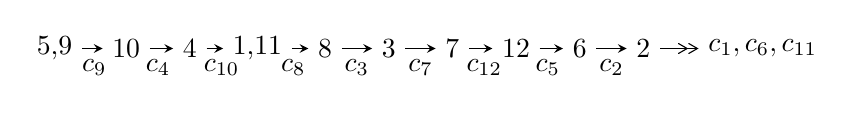
\begin{tikzpicture}[x=23pt, y=7pt]
	% node
	\node (A0) at (-1/8, 0) {5,9};
	\node (A1) at (1, 0) {10};
	\node (A2) at (2, 0) {4};
	\node (A3) at (49/16, 0) {1,11};
	\node (A4) at (33/8, 0) {8};
	\node (A5) at (41/8, 0) {3};
	\node (A6) at (49/8, 0) {7};
	\node (A7) at (57/8, 0) {12};
	\node (A8) at (65/8, 0) {6};
	\node (A9) at (73/8, 0) {2};
	\node (C1) at (1/2, -1) {$c_{9}$};
	\node (C2) at (3/2, -1) {$c_{4}$};
	\node (C3) at (5/2, -1) {$c_{10}$};
	\node (C4) at (29/8, -1) {$c_{8}$};
	\node (C5) at (37/8, -1) {$c_{3}$};
	\node (C6) at (45/8, -1) {$c_{7}$};
	\node (C7) at (53/8, -1) {$c_{12}$};
	\node (C8) at (61/8, -1) {$c_{5}$};
	\node (C9) at (69/8, -1) {$c_{2}$};
	\node (A10) at (11, 0) {$c_{1},c_{6},c_{11}$};

	% edge
	\draw[->,>=stealth]	
	(A0) edge (A1) (A1) edge (A2) (A2) edge (A3) (A3) edge (A4) (A4) edge (A5) (A5) edge (A6) (A6) edge (A7) (A7) edge (A8) (A8) edge (A9) ;
	\draw[->>,>={angle 60}]	
	(A9) edge (A10);
\end{tikzpicture} \\ 

\end{tabular} \\

\footnotetext{
The image of knot diagram is generated by the software ``\textbf{Draw programme}" developed by Andrew Bartholomew(\url{http://www.layer8.co.uk/maths/draw/index.htm\#Running-draw}), where we modified some parts for our purpose(\url{https://github.com/CATsTAILs/LinksPainter}).
}\phantom \\ \newline 
\centering \textbf{Ideals for irreducible components\footnotemark of $X_{\text{par}}$} 
 
\begin{align*}
I^u_{1}&=\langle 
6.51285\times10^{52} u^{38}+4.25612\times10^{53} u^{37}+\cdots+3.10340\times10^{55} b-6.72847\times10^{55},\\
\phantom{I^u_{1}}&\phantom{= \langle  }5.07566\times10^{53} u^{38}+1.21366\times10^{54} u^{37}+\cdots+8.27573\times10^{55} a+1.83729\times10^{55},\;u^{39}+3 u^{38}+\cdots-96 u-32\rangle \\
I^u_{2}&=\langle 
- u^{25} a- u^{25}+\cdots+6 a+43,\;-6 u^{25} a-35 u^{25}+\cdots+15 a-67,\;u^{26}- u^{25}+\cdots+u+1\rangle \\
I^u_{3}&=\langle 
u^5+b+u,\;-8 u^5+4 u^4+u^3+3 u^2+7 a-11 u+9,\;u^6+u^4+2 u^2+1\rangle \\
I^u_{4}&=\langle 
b+1,\;8 a^2-2 a u-8 a+u+1,\;u^2+2\rangle \\
\\
I^v_{1}&=\langle 
a,\;b-1,\;4 v^2+2 v+1\rangle \\
\end{align*}
\raggedright * 5 irreducible components of $\dim_{\mathbb{C}}=0$, with total 103 representations.\\
\footnotetext{All coefficients of polynomials are rational numbers. But the coefficients are sometimes approximated in decimal forms when there is not enough margin.}
\newpage
\renewcommand{\arraystretch}{1}
\centering \section*{I. $I^u_{1}= \langle 6.51\times10^{52} u^{38}+4.26\times10^{53} u^{37}+\cdots+3.10\times10^{55} b-6.73\times10^{55},\;5.08\times10^{53} u^{38}+1.21\times10^{54} u^{37}+\cdots+8.28\times10^{55} a+1.84\times10^{55},\;u^{39}+3 u^{38}+\cdots-96 u-32 \rangle$}
\flushleft \textbf{(i) Arc colorings}\\
\begin{tabular}{m{7pt} m{180pt} m{7pt} m{180pt} }
\flushright $a_{5}=$&$\begin{pmatrix}0\\u\end{pmatrix}$ \\
\flushright $a_{9}=$&$\begin{pmatrix}1\\0\end{pmatrix}$ \\
\flushright $a_{10}=$&$\begin{pmatrix}1\\u^2\end{pmatrix}$ \\
\flushright $a_{4}=$&$\begin{pmatrix}u\\u^3+u\end{pmatrix}$ \\
\flushright $a_{1}=$&$\begin{pmatrix}-0.00613319 u^{38}-0.0146653 u^{37}+\cdots-1.67950 u-0.222009\\-0.00209862 u^{38}-0.0137144 u^{37}+\cdots+4.11518 u+2.16810\end{pmatrix}$ \\
\flushright $a_{11}=$&$\begin{pmatrix}u^2+1\\u^4+2 u^2\end{pmatrix}$ \\
\flushright $a_{8}=$&$\begin{pmatrix}-0.00371852 u^{38}-0.00662758 u^{37}+\cdots-2.29660 u-0.339906\\0.00563183 u^{38}+0.0246725 u^{37}+\cdots-4.41659 u-2.14110\end{pmatrix}$ \\
\flushright $a_{3}=$&$\begin{pmatrix}0.00147024 u^{38}+0.00779912 u^{37}+\cdots-0.146149 u-0.385271\\0.0147761 u^{38}+0.0398452 u^{37}+\cdots-1.72908 u+0.367860\end{pmatrix}$ \\
\flushright $a_{7}=$&$\begin{pmatrix}-0.00248223 u^{38}+0.00407192 u^{37}+\cdots-5.63245 u-2.27061\\0.00425275 u^{38}+0.0171497 u^{37}+\cdots-2.92659 u-1.68001\end{pmatrix}$ \\
\flushright $a_{12}=$&$\begin{pmatrix}-0.00823181 u^{38}-0.0283797 u^{37}+\cdots+2.43568 u+1.94609\\-0.00209862 u^{38}-0.0137144 u^{37}+\cdots+4.11518 u+2.16810\end{pmatrix}$ \\
\flushright $a_{6}=$&$\begin{pmatrix}0.0124595 u^{38}+0.0311845 u^{37}+\cdots-1.95527 u+0.644702\\0.0123050 u^{38}+0.0359587 u^{37}+\cdots-2.29733 u+0.0612259\end{pmatrix}$ \\
\flushright $a_{2}=$&$\begin{pmatrix}-0.000124004 u^{38}-0.00169964 u^{37}+\cdots+0.337679 u+0.864298\\0.0145344 u^{38}+0.0352525 u^{37}+\cdots+0.739324 u+1.46196\end{pmatrix}$\\&\end{tabular}
\flushleft \textbf{(ii) Obstruction class $= -1$}\\~\\
\flushleft \textbf{(iii) Cusp Shapes $= 0.240650 u^{38}+0.650895 u^{37}+\cdots-36.8708 u+0.708138$}\\~\\
\newpage\renewcommand{\arraystretch}{1}
\flushleft \textbf{(iv) u-Polynomials at the component}\newline \\
\begin{tabular}{m{50pt}|m{274pt}}
Crossings & \hspace{64pt}u-Polynomials at each crossing \\
\hline $$\begin{aligned}c_{1}\end{aligned}$$&$\begin{aligned}
&u^{39}+18 u^{38}+\cdots+4081 u-576
\end{aligned}$\\
\hline $$\begin{aligned}c_{2},c_{6}\end{aligned}$$&$\begin{aligned}
&u^{39}-2 u^{38}+\cdots-7 u+24
\end{aligned}$\\
\hline $$\begin{aligned}c_{3},c_{5}\end{aligned}$$&$\begin{aligned}
&64(64 u^{39}-32 u^{38}+\cdots+42 u+7)
\end{aligned}$\\
\hline $$\begin{aligned}c_{4},c_{9},c_{10}\end{aligned}$$&$\begin{aligned}
&u^{39}-3 u^{38}+\cdots-96 u+32
\end{aligned}$\\
\hline $$\begin{aligned}c_{7},c_{8},c_{11}\\c_{12}\end{aligned}$$&$\begin{aligned}
&u^{39}-2 u^{38}+\cdots-34 u+3
\end{aligned}$\\
\hline
\end{tabular}\\~\\
\newpage\renewcommand{\arraystretch}{1}
\flushleft \textbf{(v) Riley Polynomials at the component}\newline \\
\begin{tabular}{m{50pt}|m{274pt}}
Crossings & \hspace{64pt}Riley Polynomials at each crossing \\
\hline $$\begin{aligned}c_{1}\end{aligned}$$&$\begin{aligned}
&y^{39}+10 y^{38}+\cdots+63273697 y-331776
\end{aligned}$\\
\hline $$\begin{aligned}c_{2},c_{6}\end{aligned}$$&$\begin{aligned}
&y^{39}+18 y^{38}+\cdots+4081 y-576
\end{aligned}$\\
\hline $$\begin{aligned}c_{3},c_{5}\end{aligned}$$&$\begin{aligned}
&4096(4096 y^{39}+134144 y^{38}+\cdots+294 y-49)
\end{aligned}$\\
\hline $$\begin{aligned}c_{4},c_{9},c_{10}\end{aligned}$$&$\begin{aligned}
&y^{39}+39 y^{38}+\cdots-17408 y-1024
\end{aligned}$\\
\hline $$\begin{aligned}c_{7},c_{8},c_{11}\\c_{12}\end{aligned}$$&$\begin{aligned}
&y^{39}+28 y^{38}+\cdots-32 y-9
\end{aligned}$\\
\hline
\end{tabular}\\~\\
\newpage\flushleft \textbf{(vi) Complex Volumes and Cusp Shapes}
$$\begin{array}{c|c|c}  
\text{Solutions to }I^u_{1}& \I (\text{vol} + \sqrt{-1}CS) & \text{Cusp shape}\\
 \hline 
\begin{aligned}
u &= -0.284805 + 0.928305 I \\
a &= -0.13683 - 1.42324 I \\
b &= -0.452196 + 0.700666 I\end{aligned}
 & -0.54297 + 5.03875 I & -8.25655 - 9.28786 I \\ \hline\begin{aligned}
u &= -0.284805 - 0.928305 I \\
a &= -0.13683 + 1.42324 I \\
b &= -0.452196 - 0.700666 I\end{aligned}
 & -0.54297 - 5.03875 I & -8.25655 + 9.28786 I \\ \hline\begin{aligned}
u &= \phantom{-}0.484749 + 0.961063 I \\
a &= \phantom{-}0.477652 - 0.888292 I \\
b &= -0.265156 + 0.743897 I\end{aligned}
 & -0.68459 - 2.11963 I & -9.46610 - 1.15998 I \\ \hline\begin{aligned}
u &= \phantom{-}0.484749 - 0.961063 I \\
a &= \phantom{-}0.477652 + 0.888292 I \\
b &= -0.265156 - 0.743897 I\end{aligned}
 & -0.68459 + 2.11963 I & -9.46610 + 1.15998 I \\ \hline\begin{aligned}
u &= -0.850562 + 0.700092 I \\
a &= -0.913679 - 0.827942 I \\
b &= -0.43681 + 1.39469 I\end{aligned}
 & \phantom{-}7.9219 + 13.0672 I & -2.83281 - 8.70370 I \\ \hline\begin{aligned}
u &= -0.850562 - 0.700092 I \\
a &= -0.913679 + 0.827942 I \\
b &= -0.43681 - 1.39469 I\end{aligned}
 & \phantom{-}7.9219 - 13.0672 I & -2.83281 + 8.70370 I \\ \hline\begin{aligned}
u &= \phantom{-}0.021011 + 1.113620 I \\
a &= \phantom{-}0.113149 + 0.982543 I \\
b &= -0.417378 - 0.585720 I\end{aligned}
 & \phantom{-}2.61415 - 1.46386 I & -3.75938 + 4.77609 I \\ \hline\begin{aligned}
u &= \phantom{-}0.021011 - 1.113620 I \\
a &= \phantom{-}0.113149 - 0.982543 I \\
b &= -0.417378 + 0.585720 I\end{aligned}
 & \phantom{-}2.61415 + 1.46386 I & -3.75938 - 4.77609 I \\ \hline\begin{aligned}
u &= -1.024080 + 0.504017 I \\
a &= -0.340192 - 0.350015 I \\
b &= \phantom{-}0.242441 + 1.346780 I\end{aligned}
 & \phantom{-}7.21089 - 6.95675 I & -1.57897 + 4.70182 I \\ \hline\begin{aligned}
u &= -1.024080 - 0.504017 I \\
a &= -0.340192 + 0.350015 I \\
b &= \phantom{-}0.242441 - 1.346780 I\end{aligned}
 & \phantom{-}7.21089 + 6.95675 I & -1.57897 - 4.70182 I\\
 \hline 
 \end{array}$$\newpage$$\begin{array}{c|c|c}  
\text{Solutions to }I^u_{1}& \I (\text{vol} + \sqrt{-1}CS) & \text{Cusp shape}\\
 \hline 
\begin{aligned}
u &= \phantom{-}0.899466 + 0.710929 I \\
a &= -0.806485 + 0.746074 I \\
b &= -0.31980 - 1.40480 I\end{aligned}
 & \phantom{-}9.60981 - 6.62935 I & -0.44294 + 4.43297 I \\ \hline\begin{aligned}
u &= \phantom{-}0.899466 - 0.710929 I \\
a &= -0.806485 - 0.746074 I \\
b &= -0.31980 + 1.40480 I\end{aligned}
 & \phantom{-}9.60981 + 6.62935 I & -0.44294 - 4.43297 I \\ \hline\begin{aligned}
u &= \phantom{-}1.046090 + 0.585321 I \\
a &= -0.447106 + 0.457880 I \\
b &= \phantom{-}0.097717 - 1.375450 I\end{aligned}
 & \phantom{-}9.08947 + 0.21395 I & \phantom{-}1.186596 + 0.413950 I \\ \hline\begin{aligned}
u &= \phantom{-}1.046090 - 0.585321 I \\
a &= -0.447106 - 0.457880 I \\
b &= \phantom{-}0.097717 + 1.375450 I\end{aligned}
 & \phantom{-}9.08947 - 0.21395 I & \phantom{-}1.186596 - 0.413950 I \\ \hline\begin{aligned}
u &= -1.088540 + 0.802120 I \\
a &= -0.469791 - 0.757971 I \\
b &= -0.104038 + 1.220040 I\end{aligned}
 & \phantom{-}1.35178 + 3.70831 I & \phantom{-0.000000 } 0. - 5.50700 I \\ \hline\begin{aligned}
u &= -1.088540 - 0.802120 I \\
a &= -0.469791 + 0.757971 I \\
b &= -0.104038 - 1.220040 I\end{aligned}
 & \phantom{-}1.35178 - 3.70831 I & \phantom{-0.000000 -}0. + 5.50700 I \\ \hline\begin{aligned}
u &= \phantom{-}0.024809 + 1.389690 I \\
a &= -0.682113 + 0.285569 I \\
b &= -0.128700 - 0.137181 I\end{aligned}
 & \phantom{-}4.95731 - 2.14817 I & \phantom{-0.000000 -}0. + 4.01911 I \\ \hline\begin{aligned}
u &= \phantom{-}0.024809 - 1.389690 I \\
a &= -0.682113 - 0.285569 I \\
b &= -0.128700 + 0.137181 I\end{aligned}
 & \phantom{-}4.95731 + 2.14817 I & \phantom{-0.000000 } 0. - 4.01911 I \\ \hline\begin{aligned}
u &= -0.087825 + 1.410570 I \\
a &= \phantom{-}0.565414 + 0.372983 I \\
b &= -0.993287 - 0.445251 I\end{aligned}
 & \phantom{-}2.42149 - 0.42416 I & -8.00000 + 0. I\phantom{ +0.000000I} \\ \hline\begin{aligned}
u &= -0.087825 - 1.410570 I \\
a &= \phantom{-}0.565414 - 0.372983 I \\
b &= -0.993287 + 0.445251 I\end{aligned}
 & \phantom{-}2.42149 + 0.42416 I & -8.00000 + 0. I\phantom{ +0.000000I}\\
 \hline 
 \end{array}$$\newpage$$\begin{array}{c|c|c}  
\text{Solutions to }I^u_{1}& \I (\text{vol} + \sqrt{-1}CS) & \text{Cusp shape}\\
 \hline 
\begin{aligned}
u &= -0.475767 + 0.181696 I \\
a &= \phantom{-}0.383979 - 0.039197 I \\
b &= \phantom{-}0.773750 + 0.480261 I\end{aligned}
 & -2.68424 - 2.19929 I & -15.6702 + 1.3086 I \\ \hline\begin{aligned}
u &= -0.475767 - 0.181696 I \\
a &= \phantom{-}0.383979 + 0.039197 I \\
b &= \phantom{-}0.773750 - 0.480261 I\end{aligned}
 & -2.68424 + 2.19929 I & -15.6702 - 1.3086 I \\ \hline\begin{aligned}
u &= -0.01764 + 1.52619 I \\
a &= \phantom{-}0.955880 + 0.065318 I \\
b &= -1.64994 - 0.11450 I\end{aligned}
 & \phantom{-}5.17213 + 2.58745 I & \phantom{-0.000000 } 0 \\ \hline\begin{aligned}
u &= -0.01764 - 1.52619 I \\
a &= \phantom{-}0.955880 - 0.065318 I \\
b &= -1.64994 + 0.11450 I\end{aligned}
 & \phantom{-}5.17213 - 2.58745 I & \phantom{-0.000000 } 0 \\ \hline\begin{aligned}
u &= \phantom{-}0.071403 + 0.441330 I \\
a &= \phantom{-}1.51732 - 0.80229 I \\
b &= -0.338553 + 0.229132 I\end{aligned}
 & -0.54939 - 1.65860 I & -4.21380 + 1.79570 I \\ \hline\begin{aligned}
u &= \phantom{-}0.071403 - 0.441330 I \\
a &= \phantom{-}1.51732 + 0.80229 I \\
b &= -0.338553 - 0.229132 I\end{aligned}
 & -0.54939 + 1.65860 I & -4.21380 - 1.79570 I \\ \hline\begin{aligned}
u &= -0.094781 + 0.360218 I \\
a &= \phantom{-}0.544712 + 0.036408 I \\
b &= \phantom{-}1.215470 + 0.103619 I\end{aligned}
 & -1.37228 + 2.24874 I & \phantom{-}4.40609 - 10.02980 I \\ \hline\begin{aligned}
u &= -0.094781 - 0.360218 I \\
a &= \phantom{-}0.544712 - 0.036408 I \\
b &= \phantom{-}1.215470 - 0.103619 I\end{aligned}
 & -1.37228 - 2.24874 I & \phantom{-}4.40609 + 10.02980 I \\ \hline\begin{aligned}
u &= \phantom{-}0.372322\phantom{ +0.000000I} \\
a &= \phantom{-}0.597491\phantom{ +0.000000I} \\
b &= \phantom{-}0.434285\phantom{ +0.000000I}\end{aligned}
 & -0.672199\phantom{ +0.000000I} & -14.5900\phantom{ +0.000000I} \\ \hline\begin{aligned}
u &= -0.27857 + 1.61370 I \\
a &= \phantom{-}0.62986 + 1.83200 I \\
b &= \phantom{-}0.56880 - 1.49325 I\end{aligned}
 & \phantom{-}15.5418 + 17.2782 I & \phantom{-0.000000 } 0\\
 \hline 
 \end{array}$$\newpage$$\begin{array}{c|c|c}  
\text{Solutions to }I^u_{1}& \I (\text{vol} + \sqrt{-1}CS) & \text{Cusp shape}\\
 \hline 
\begin{aligned}
u &= -0.27857 - 1.61370 I \\
a &= \phantom{-}0.62986 - 1.83200 I \\
b &= \phantom{-}0.56880 + 1.49325 I\end{aligned}
 & \phantom{-}15.5418 - 17.2782 I & \phantom{-0.000000 } 0 \\ \hline\begin{aligned}
u &= \phantom{-}0.28827 + 1.62593 I \\
a &= \phantom{-}0.62219 - 1.76672 I \\
b &= \phantom{-}0.48592 + 1.51538 I\end{aligned}
 & \phantom{-}17.3108 - 11.0467 I & \phantom{-0.000000 } 0 \\ \hline\begin{aligned}
u &= \phantom{-}0.28827 - 1.62593 I \\
a &= \phantom{-}0.62219 + 1.76672 I \\
b &= \phantom{-}0.48592 - 1.51538 I\end{aligned}
 & \phantom{-}17.3108 + 11.0467 I & \phantom{-0.000000 } 0 \\ \hline\begin{aligned}
u &= -0.27452 + 1.67561 I \\
a &= \phantom{-}0.45265 + 1.68686 I \\
b &= \phantom{-}0.351061 - 1.346420 I\end{aligned}
 & \phantom{-}9.74081 + 8.64375 I & \phantom{-0.000000 } 0 \\ \hline\begin{aligned}
u &= -0.27452 - 1.67561 I \\
a &= \phantom{-}0.45265 - 1.68686 I \\
b &= \phantom{-}0.351061 + 1.346420 I\end{aligned}
 & \phantom{-}9.74081 - 8.64375 I & \phantom{-0.000000 } 0 \\ \hline\begin{aligned}
u &= \phantom{-}0.34143 + 1.66879 I \\
a &= \phantom{-}0.56308 - 1.50519 I \\
b &= \phantom{-}0.14914 + 1.47169 I\end{aligned}
 & \phantom{-}16.5682 - 5.0648 I & \phantom{-0.000000 } 0 \\ \hline\begin{aligned}
u &= \phantom{-}0.34143 - 1.66879 I \\
a &= \phantom{-}0.56308 + 1.50519 I \\
b &= \phantom{-}0.14914 - 1.47169 I\end{aligned}
 & \phantom{-}16.5682 + 5.0648 I & \phantom{-0.000000 } 0 \\ \hline\begin{aligned}
u &= -0.38631 + 1.66978 I \\
a &= \phantom{-}0.54657 + 1.37900 I \\
b &= \phantom{-}0.00441 - 1.41697 I\end{aligned}
 & \phantom{-}14.2718 - 1.5060 I & \phantom{-0.000000 } 0 \\ \hline\begin{aligned}
u &= -0.38631 - 1.66978 I \\
a &= \phantom{-}0.54657 - 1.37900 I \\
b &= \phantom{-}0.00441 + 1.41697 I\end{aligned}
 & \phantom{-}14.2718 + 1.5060 I & \phantom{-0.000000 } 0\\
 \hline 
 \end{array}$$\newpage\newpage\renewcommand{\arraystretch}{1}
\centering \section*{II. $I^u_{2}= \langle - u^{25} a- u^{25}+\cdots+6 a+43,\;-6 u^{25} a-35 u^{25}+\cdots+15 a-67,\;u^{26}- u^{25}+\cdots+u+1 \rangle$}
\flushleft \textbf{(i) Arc colorings}\\
\begin{tabular}{m{7pt} m{180pt} m{7pt} m{180pt} }
\flushright $a_{5}=$&$\begin{pmatrix}0\\u\end{pmatrix}$ \\
\flushright $a_{9}=$&$\begin{pmatrix}1\\0\end{pmatrix}$ \\
\flushright $a_{10}=$&$\begin{pmatrix}1\\u^2\end{pmatrix}$ \\
\flushright $a_{4}=$&$\begin{pmatrix}u\\u^3+u\end{pmatrix}$ \\
\flushright $a_{1}=$&$\begin{pmatrix}a\\0.0270270 a u^{25}+0.0270270 u^{25}+\cdots-0.162162 a-1.16216\end{pmatrix}$ \\
\flushright $a_{11}=$&$\begin{pmatrix}u^2+1\\u^4+2 u^2\end{pmatrix}$ \\
\flushright $a_{8}=$&$\begin{pmatrix}0.0270270 a u^{25}+1.36036 u^{25}+\cdots-1.16216 a-0.495495\\0.0270270 a u^{25}+0.0270270 u^{25}+\cdots-0.162162 a+0.837838\end{pmatrix}$ \\
\flushright $a_{3}=$&$\begin{pmatrix}0.990991 a u^{25}-0.453453 u^{25}+\cdots+1.38739 a+2.16517\\0.486486 a u^{25}-0.846847 u^{25}+\cdots+0.0810811 a-0.585586\end{pmatrix}$ \\
\flushright $a_{7}=$&$\begin{pmatrix}0.0270270 a u^{25}+1.36036 u^{25}+\cdots-1.16216 a-1.49550\\1\end{pmatrix}$ \\
\flushright $a_{12}=$&$\begin{pmatrix}0.0270270 a u^{25}+0.0270270 u^{25}+\cdots+0.837838 a-1.16216\\0.0270270 a u^{25}+0.0270270 u^{25}+\cdots-0.162162 a-1.16216\end{pmatrix}$ \\
\flushright $a_{6}=$&$\begin{pmatrix}0.846847 a u^{25}-1.04204 u^{25}+\cdots+0.585586 a+1.14114\\-0.324324 a u^{25}-0.990991 u^{25}+\cdots-0.0540541 a-1.38739\end{pmatrix}$ \\
\flushright $a_{2}=$&$\begin{pmatrix}-0.774775 a u^{25}-0.330330 u^{25}+\cdots+2.31532 a-1.46246\\-0.135135 a u^{25}-0.801802 u^{25}+\cdots+0.810811 a-1.52252\end{pmatrix}$\\&\end{tabular}
\flushleft \textbf{(ii) Obstruction class $= -1$}\\~\\
\flushleft \textbf{(iii) Cusp Shapes $= 4 u^{24}-4 u^{23}+56 u^{22}-52 u^{21}+332 u^{20}-284 u^{19}+1080 u^{18}-844 u^{17}+2096 u^{16}-1484 u^{15}+2508 u^{14}-1596 u^{13}+1940 u^{12}-1096 u^{11}+1112 u^{10}-540 u^9+504 u^8-212 u^7+132 u^6-60 u^5+48 u^4-12 u^3+16 u^2-12 u-6$}\\~\\
\newpage\renewcommand{\arraystretch}{1}
\flushleft \textbf{(iv) u-Polynomials at the component}\newline \\
\begin{tabular}{m{50pt}|m{274pt}}
Crossings & \hspace{64pt}u-Polynomials at each crossing \\
\hline $$\begin{aligned}c_{1}\end{aligned}$$&$\begin{aligned}
&(u^{26}+9 u^{25}+\cdots+5 u+1)^{2}
\end{aligned}$\\
\hline $$\begin{aligned}c_{2},c_{6}\end{aligned}$$&$\begin{aligned}
&(u^{26}- u^{25}+\cdots- u+1)^{2}
\end{aligned}$\\
\hline $$\begin{aligned}c_{3},c_{5}\end{aligned}$$&$\begin{aligned}
&9(9 u^{52}-87 u^{51}+\cdots-3.27654\times10^{7} u+6443297)
\end{aligned}$\\
\hline $$\begin{aligned}c_{4},c_{9},c_{10}\end{aligned}$$&$\begin{aligned}
&(u^{26}+u^{25}+\cdots- u+1)^{2}
\end{aligned}$\\
\hline $$\begin{aligned}c_{7},c_{8},c_{11}\\c_{12}\end{aligned}$$&$\begin{aligned}
&u^{52}+5 u^{51}+\cdots+548 u+125
\end{aligned}$\\
\hline
\end{tabular}\\~\\
\newpage\renewcommand{\arraystretch}{1}
\flushleft \textbf{(v) Riley Polynomials at the component}\newline \\
\begin{tabular}{m{50pt}|m{274pt}}
Crossings & \hspace{64pt}Riley Polynomials at each crossing \\
\hline $$\begin{aligned}c_{1}\end{aligned}$$&$\begin{aligned}
&(y^{26}+17 y^{25}+\cdots+29 y+1)^{2}
\end{aligned}$\\
\hline $$\begin{aligned}c_{2},c_{6}\end{aligned}$$&$\begin{aligned}
&(y^{26}+9 y^{25}+\cdots+5 y+1)^{2}
\end{aligned}$\\
\hline $$\begin{aligned}c_{3},c_{5}\end{aligned}$$&$\begin{aligned}
&81\\
&\cdot(81 y^{52}+2835 y^{51}+\cdots+516271175779380 y+41516076230209)
\end{aligned}$\\
\hline $$\begin{aligned}c_{4},c_{9},c_{10}\end{aligned}$$&$\begin{aligned}
&(y^{26}+29 y^{25}+\cdots+5 y+1)^{2}
\end{aligned}$\\
\hline $$\begin{aligned}c_{7},c_{8},c_{11}\\c_{12}\end{aligned}$$&$\begin{aligned}
&y^{52}+39 y^{51}+\cdots+151696 y+15625
\end{aligned}$\\
\hline
\end{tabular}\\~\\
\newpage\flushleft \textbf{(vi) Complex Volumes and Cusp Shapes}
$$\begin{array}{c|c|c}  
\text{Solutions to }I^u_{2}& \I (\text{vol} + \sqrt{-1}CS) & \text{Cusp shape}\\
 \hline 
\begin{aligned}
u &= \phantom{-}0.557205 + 0.605601 I \\
a &= \phantom{-}0.908515 - 0.786612 I \\
b &= \phantom{-}0.44461 + 1.37915 I\end{aligned}
 & \phantom{-}3.14131 - 7.92757 I & -5.52051 + 8.33110 I \\ \hline\begin{aligned}
u &= \phantom{-}0.557205 + 0.605601 I \\
a &= -0.546617 + 0.149415 I \\
b &= -1.009470 - 0.105339 I\end{aligned}
 & \phantom{-}3.14131 - 7.92757 I & -5.52051 + 8.33110 I \\ \hline\begin{aligned}
u &= \phantom{-}0.557205 - 0.605601 I \\
a &= \phantom{-}0.908515 + 0.786612 I \\
b &= \phantom{-}0.44461 - 1.37915 I\end{aligned}
 & \phantom{-}3.14131 + 7.92757 I & -5.52051 - 8.33110 I \\ \hline\begin{aligned}
u &= \phantom{-}0.557205 - 0.605601 I \\
a &= -0.546617 - 0.149415 I \\
b &= -1.009470 + 0.105339 I\end{aligned}
 & \phantom{-}3.14131 + 7.92757 I & -5.52051 - 8.33110 I \\ \hline\begin{aligned}
u &= -0.063283 + 0.808616 I \\
a &= -0.774190 + 0.526907 I \\
b &= -0.406074 - 1.296320 I\end{aligned}
 & \phantom{-}7.01322 + 2.64715 I & \phantom{-}0.54618 - 3.67555 I \\ \hline\begin{aligned}
u &= -0.063283 + 0.808616 I \\
a &= -1.113660 - 0.448597 I \\
b &= -0.481799 + 1.224650 I\end{aligned}
 & \phantom{-}7.01322 + 2.64715 I & \phantom{-}0.54618 - 3.67555 I \\ \hline\begin{aligned}
u &= -0.063283 - 0.808616 I \\
a &= -0.774190 - 0.526907 I \\
b &= -0.406074 + 1.296320 I\end{aligned}
 & \phantom{-}7.01322 - 2.64715 I & \phantom{-}0.54618 + 3.67555 I \\ \hline\begin{aligned}
u &= -0.063283 - 0.808616 I \\
a &= -1.113660 + 0.448597 I \\
b &= -0.481799 - 1.224650 I\end{aligned}
 & \phantom{-}7.01322 - 2.64715 I & \phantom{-}0.54618 + 3.67555 I \\ \hline\begin{aligned}
u &= -0.506771 + 0.602442 I \\
a &= \phantom{-}0.845502 + 0.826551 I \\
b &= \phantom{-}0.283417 - 1.369520 I\end{aligned}
 & \phantom{-}4.26499 + 2.50037 I & -3.37218 - 3.68649 I \\ \hline\begin{aligned}
u &= -0.506771 + 0.602442 I \\
a &= -0.706203 - 0.001643 I \\
b &= -0.857226 + 0.277909 I\end{aligned}
 & \phantom{-}4.26499 + 2.50037 I & -3.37218 - 3.68649 I\\
 \hline 
 \end{array}$$\newpage$$\begin{array}{c|c|c}  
\text{Solutions to }I^u_{2}& \I (\text{vol} + \sqrt{-1}CS) & \text{Cusp shape}\\
 \hline 
\begin{aligned}
u &= -0.506771 - 0.602442 I \\
a &= \phantom{-}0.845502 - 0.826551 I \\
b &= \phantom{-}0.283417 + 1.369520 I\end{aligned}
 & \phantom{-}4.26499 - 2.50037 I & -3.37218 + 3.68649 I \\ \hline\begin{aligned}
u &= -0.506771 - 0.602442 I \\
a &= -0.706203 + 0.001643 I \\
b &= -0.857226 - 0.277909 I\end{aligned}
 & \phantom{-}4.26499 - 2.50037 I & -3.37218 + 3.68649 I \\ \hline\begin{aligned}
u &= \phantom{-}0.565256 + 0.486664 I \\
a &= \phantom{-}0.876953 - 0.806174 I \\
b &= \phantom{-}0.315896 + 0.901619 I\end{aligned}
 & -1.29717 - 1.94179 I & -11.39486 + 3.84898 I \\ \hline\begin{aligned}
u &= \phantom{-}0.565256 + 0.486664 I \\
a &= \phantom{-}0.023979 - 0.302536 I \\
b &= -0.446412 + 0.289709 I\end{aligned}
 & -1.29717 - 1.94179 I & -11.39486 + 3.84898 I \\ \hline\begin{aligned}
u &= \phantom{-}0.565256 - 0.486664 I \\
a &= \phantom{-}0.876953 + 0.806174 I \\
b &= \phantom{-}0.315896 - 0.901619 I\end{aligned}
 & -1.29717 + 1.94179 I & -11.39486 - 3.84898 I \\ \hline\begin{aligned}
u &= \phantom{-}0.565256 - 0.486664 I \\
a &= \phantom{-}0.023979 + 0.302536 I \\
b &= -0.446412 - 0.289709 I\end{aligned}
 & -1.29717 + 1.94179 I & -11.39486 - 3.84898 I \\ \hline\begin{aligned}
u &= \phantom{-}0.588033 + 0.339866 I \\
a &= \phantom{-}1.354340 + 0.197426 I \\
b &= -0.190825 + 1.201440 I\end{aligned}
 & \phantom{-}2.36739 + 4.00629 I & -7.77829 - 2.28167 I \\ \hline\begin{aligned}
u &= \phantom{-}0.588033 + 0.339866 I \\
a &= \phantom{-}0.52368 - 1.59827 I \\
b &= \phantom{-}0.544635 - 0.217951 I\end{aligned}
 & \phantom{-}2.36739 + 4.00629 I & -7.77829 - 2.28167 I \\ \hline\begin{aligned}
u &= \phantom{-}0.588033 - 0.339866 I \\
a &= \phantom{-}1.354340 - 0.197426 I \\
b &= -0.190825 - 1.201440 I\end{aligned}
 & \phantom{-}2.36739 - 4.00629 I & -7.77829 + 2.28167 I \\ \hline\begin{aligned}
u &= \phantom{-}0.588033 - 0.339866 I \\
a &= \phantom{-}0.52368 + 1.59827 I \\
b &= \phantom{-}0.544635 + 0.217951 I\end{aligned}
 & \phantom{-}2.36739 - 4.00629 I & -7.77829 + 2.28167 I\\
 \hline 
 \end{array}$$\newpage$$\begin{array}{c|c|c}  
\text{Solutions to }I^u_{2}& \I (\text{vol} + \sqrt{-1}CS) & \text{Cusp shape}\\
 \hline 
\begin{aligned}
u &= -0.489623 + 0.284759 I \\
a &= \phantom{-}2.18275 + 0.11119 I \\
b &= -0.014701 - 1.195450 I\end{aligned}
 & \phantom{-}3.40411 + 1.00551 I & -6.42231 - 3.62739 I \\ \hline\begin{aligned}
u &= -0.489623 + 0.284759 I \\
a &= \phantom{-}0.06160 + 2.26036 I \\
b &= \phantom{-}0.279398 + 0.549276 I\end{aligned}
 & \phantom{-}3.40411 + 1.00551 I & -6.42231 - 3.62739 I \\ \hline\begin{aligned}
u &= -0.489623 - 0.284759 I \\
a &= \phantom{-}2.18275 - 0.11119 I \\
b &= -0.014701 + 1.195450 I\end{aligned}
 & \phantom{-}3.40411 - 1.00551 I & -6.42231 + 3.62739 I \\ \hline\begin{aligned}
u &= -0.489623 - 0.284759 I \\
a &= \phantom{-}0.06160 - 2.26036 I \\
b &= \phantom{-}0.279398 - 0.549276 I\end{aligned}
 & \phantom{-}3.40411 - 1.00551 I & -6.42231 + 3.62739 I \\ \hline\begin{aligned}
u &= \phantom{-}0.08778 + 1.44888 I \\
a &= \phantom{-}1.36031 + 0.96993 I \\
b &= \phantom{-}0.123022 + 0.607999 I\end{aligned}
 & \phantom{-}7.95687 + 1.77746 I & -4.37085 - 2.67865 I \\ \hline\begin{aligned}
u &= \phantom{-}0.08778 + 1.44888 I \\
a &= -1.67018 + 2.70770 I \\
b &= \phantom{-}0.003774 - 1.163280 I\end{aligned}
 & \phantom{-}7.95687 + 1.77746 I & -4.37085 - 2.67865 I \\ \hline\begin{aligned}
u &= \phantom{-}0.08778 - 1.44888 I \\
a &= \phantom{-}1.36031 - 0.96993 I \\
b &= \phantom{-}0.123022 - 0.607999 I\end{aligned}
 & \phantom{-}7.95687 - 1.77746 I & -4.37085 + 2.67865 I \\ \hline\begin{aligned}
u &= \phantom{-}0.08778 - 1.44888 I \\
a &= -1.67018 - 2.70770 I \\
b &= \phantom{-}0.003774 + 1.163280 I\end{aligned}
 & \phantom{-}7.95687 - 1.77746 I & -4.37085 + 2.67865 I \\ \hline\begin{aligned}
u &= -0.304550 + 0.390095 I \\
a &= -2.14676 + 1.48082 I \\
b &= -0.147408 + 0.712500 I\end{aligned}
 & \phantom{-}3.22784 + 0.99254 I & -5.03716 - 6.67512 I \\ \hline\begin{aligned}
u &= -0.304550 + 0.390095 I \\
a &= \phantom{-}1.58906 + 2.18030 I \\
b &= -0.024365 - 1.159480 I\end{aligned}
 & \phantom{-}3.22784 + 0.99254 I & -5.03716 - 6.67512 I\\
 \hline 
 \end{array}$$\newpage$$\begin{array}{c|c|c}  
\text{Solutions to }I^u_{2}& \I (\text{vol} + \sqrt{-1}CS) & \text{Cusp shape}\\
 \hline 
\begin{aligned}
u &= -0.304550 - 0.390095 I \\
a &= -2.14676 - 1.48082 I \\
b &= -0.147408 - 0.712500 I\end{aligned}
 & \phantom{-}3.22784 - 0.99254 I & -5.03716 + 6.67512 I \\ \hline\begin{aligned}
u &= -0.304550 - 0.390095 I \\
a &= \phantom{-}1.58906 - 2.18030 I \\
b &= -0.024365 + 1.159480 I\end{aligned}
 & \phantom{-}3.22784 - 0.99254 I & -5.03716 + 6.67512 I \\ \hline\begin{aligned}
u &= \phantom{-}0.15393 + 1.51610 I \\
a &= -0.244659 + 0.073372 I \\
b &= \phantom{-}0.781532 + 0.034297 I\end{aligned}
 & \phantom{-}5.31067 - 4.47678 I & -7.30340 + 3.58620 I \\ \hline\begin{aligned}
u &= \phantom{-}0.15393 + 1.51610 I \\
a &= -0.51526 + 1.89761 I \\
b &= -0.374114 - 1.224410 I\end{aligned}
 & \phantom{-}5.31067 - 4.47678 I & -7.30340 + 3.58620 I \\ \hline\begin{aligned}
u &= \phantom{-}0.15393 - 1.51610 I \\
a &= -0.244659 - 0.073372 I \\
b &= \phantom{-}0.781532 - 0.034297 I\end{aligned}
 & \phantom{-}5.31067 + 4.47678 I & -7.30340 - 3.58620 I \\ \hline\begin{aligned}
u &= \phantom{-}0.15393 - 1.51610 I \\
a &= -0.51526 - 1.89761 I \\
b &= -0.374114 + 1.224410 I\end{aligned}
 & \phantom{-}5.31067 + 4.47678 I & -7.30340 - 3.58620 I \\ \hline\begin{aligned}
u &= -0.09394 + 1.52190 I \\
a &= \phantom{-}0.460645 + 0.452308 I \\
b &= \phantom{-}0.665565 - 0.626074 I\end{aligned}
 & \phantom{-}9.71769 + 2.46970 I & -0.41193 - 2.77943 I \\ \hline\begin{aligned}
u &= -0.09394 + 1.52190 I \\
a &= -0.45078 - 2.30789 I \\
b &= -0.038145 + 1.373730 I\end{aligned}
 & \phantom{-}9.71769 + 2.46970 I & -0.41193 - 2.77943 I \\ \hline\begin{aligned}
u &= -0.09394 - 1.52190 I \\
a &= \phantom{-}0.460645 - 0.452308 I \\
b &= \phantom{-}0.665565 + 0.626074 I\end{aligned}
 & \phantom{-}9.71769 - 2.46970 I & -0.41193 + 2.77943 I \\ \hline\begin{aligned}
u &= -0.09394 - 1.52190 I \\
a &= -0.45078 + 2.30789 I \\
b &= -0.038145 - 1.373730 I\end{aligned}
 & \phantom{-}9.71769 - 2.46970 I & -0.41193 + 2.77943 I\\
 \hline 
 \end{array}$$\newpage$$\begin{array}{c|c|c}  
\text{Solutions to }I^u_{2}& \I (\text{vol} + \sqrt{-1}CS) & \text{Cusp shape}\\
 \hline 
\begin{aligned}
u &= -0.14965 + 1.56671 I \\
a &= -0.427513 + 0.464073 I \\
b &= \phantom{-}1.286740 - 0.289716 I\end{aligned}
 & \phantom{-}11.55040 + 4.90123 I & -0.29851 - 2.20839 I \\ \hline\begin{aligned}
u &= -0.14965 + 1.56671 I \\
a &= -0.33833 - 2.00964 I \\
b &= -0.45547 + 1.63285 I\end{aligned}
 & \phantom{-}11.55040 + 4.90123 I & -0.29851 - 2.20839 I \\ \hline\begin{aligned}
u &= -0.14965 - 1.56671 I \\
a &= -0.427513 - 0.464073 I \\
b &= \phantom{-}1.286740 + 0.289716 I\end{aligned}
 & \phantom{-}11.55040 - 4.90123 I & -0.29851 + 2.20839 I \\ \hline\begin{aligned}
u &= -0.14965 - 1.56671 I \\
a &= -0.33833 + 2.00964 I \\
b &= -0.45547 - 1.63285 I\end{aligned}
 & \phantom{-}11.55040 - 4.90123 I & -0.29851 + 2.20839 I \\ \hline\begin{aligned}
u &= \phantom{-}0.16684 + 1.56649 I \\
a &= -0.567065 - 0.388686 I \\
b &= \phantom{-}1.367540 + 0.115693 I\end{aligned}
 & \phantom{-}10.4089 - 10.5785 I & -2.23924 + 6.94484 I \\ \hline\begin{aligned}
u &= \phantom{-}0.16684 + 1.56649 I \\
a &= -0.31601 + 1.97598 I \\
b &= -0.60715 - 1.60654 I\end{aligned}
 & \phantom{-}10.4089 - 10.5785 I & -2.23924 + 6.94484 I \\ \hline\begin{aligned}
u &= \phantom{-}0.16684 - 1.56649 I \\
a &= -0.567065 + 0.388686 I \\
b &= \phantom{-}1.367540 - 0.115693 I\end{aligned}
 & \phantom{-}10.4089 + 10.5785 I & -2.23924 - 6.94484 I \\ \hline\begin{aligned}
u &= \phantom{-}0.16684 - 1.56649 I \\
a &= -0.31601 - 1.97598 I \\
b &= -0.60715 + 1.60654 I\end{aligned}
 & \phantom{-}10.4089 + 10.5785 I & -2.23924 - 6.94484 I \\ \hline\begin{aligned}
u &= -0.01123 + 1.60251 I \\
a &= -0.09006 + 1.65768 I \\
b &= \phantom{-}0.80517 - 1.55246 I\end{aligned}
 & \phantom{-}15.1804 + 2.8815 I & \phantom{-}1.60306 - 2.87824 I \\ \hline\begin{aligned}
u &= -0.01123 + 1.60251 I \\
a &= -0.11338 - 1.79936 I \\
b &= \phantom{-}0.65186 + 1.66532 I\end{aligned}
 & \phantom{-}15.1804 + 2.8815 I & \phantom{-}1.60306 - 2.87824 I\\
 \hline 
 \end{array}$$\newpage$$\begin{array}{c|c|c}  
\text{Solutions to }I^u_{2}& \I (\text{vol} + \sqrt{-1}CS) & \text{Cusp shape}\\
 \hline 
\begin{aligned}
u &= -0.01123 - 1.60251 I \\
a &= -0.09006 - 1.65768 I \\
b &= \phantom{-}0.80517 + 1.55246 I\end{aligned}
 & \phantom{-}15.1804 - 2.8815 I & \phantom{-}1.60306 + 2.87824 I \\ \hline\begin{aligned}
u &= -0.01123 - 1.60251 I \\
a &= -0.11338 + 1.79936 I \\
b &= \phantom{-}0.65186 - 1.66532 I\end{aligned}
 & \phantom{-}15.1804 - 2.8815 I & \phantom{-}1.60306 + 2.87824 I\\
 \hline 
 \end{array}$$\newpage\newpage\renewcommand{\arraystretch}{1}
\centering \section*{III. $I^u_{3}= \langle u^5+b+u,\;-8 u^5+4 u^4+u^3+3 u^2+7 a-11 u+9,\;u^6+u^4+2 u^2+1 \rangle$}
\flushleft \textbf{(i) Arc colorings}\\
\begin{tabular}{m{7pt} m{180pt} m{7pt} m{180pt} }
\flushright $a_{5}=$&$\begin{pmatrix}0\\u\end{pmatrix}$ \\
\flushright $a_{9}=$&$\begin{pmatrix}1\\0\end{pmatrix}$ \\
\flushright $a_{10}=$&$\begin{pmatrix}1\\u^2\end{pmatrix}$ \\
\flushright $a_{4}=$&$\begin{pmatrix}u\\u^3+u\end{pmatrix}$ \\
\flushright $a_{1}=$&$\begin{pmatrix}\frac{8}{7} u^5-\frac{4}{7} u^4+\cdots+\frac{11}{7} u-\frac{9}{7}\\- u^5- u\end{pmatrix}$ \\
\flushright $a_{11}=$&$\begin{pmatrix}u^2+1\\u^4+2 u^2\end{pmatrix}$ \\
\flushright $a_{8}=$&$\begin{pmatrix}-\frac{6}{7} u^5-\frac{3}{7} u^4+\cdots-\frac{10}{7} u-\frac{5}{7}\\1\end{pmatrix}$ \\
\flushright $a_{3}=$&$\begin{pmatrix}-\frac{29}{49} u^4-\frac{6}{49} u^2+u-\frac{60}{49}\\-\frac{4}{7} u^5+\frac{2}{7} u^4+\cdots-\frac{2}{7} u+\frac{1}{7}\end{pmatrix}$ \\
\flushright $a_{7}=$&$\begin{pmatrix}-\frac{6}{7} u^5-\frac{3}{7} u^4+\cdots-\frac{10}{7} u-\frac{5}{7}\\2 u^5+u^3+u+1\end{pmatrix}$ \\
\flushright $a_{12}=$&$\begin{pmatrix}\frac{1}{7} u^5-\frac{4}{7} u^4+\cdots+\frac{4}{7} u-\frac{9}{7}\\- u^5- u\end{pmatrix}$ \\
\flushright $a_{6}=$&$\begin{pmatrix}-\frac{4}{7} u^5-\frac{20}{49} u^4+\cdots-\frac{9}{7} u-\frac{38}{49}\\-\frac{3}{7} u^5+\frac{5}{7} u^4+\cdots+\frac{2}{7} u+\frac{6}{7}\end{pmatrix}$ \\
\flushright $a_{2}=$&$\begin{pmatrix}\frac{1}{7} u^5-\frac{3}{49} u^4+\cdots+\frac{11}{7} u-\frac{40}{49}\\-\frac{5}{7} u^5-\frac{1}{7} u^4+\cdots+\frac{1}{7} u-\frac{4}{7}\end{pmatrix}$\\&\end{tabular}
\flushleft \textbf{(ii) Obstruction class $= 1$}\\~\\
\flushleft \textbf{(iii) Cusp Shapes $= 4 u^4+4 u^2+4$}\\~\\
\newpage\renewcommand{\arraystretch}{1}
\flushleft \textbf{(iv) u-Polynomials at the component}\newline \\
\begin{tabular}{m{50pt}|m{274pt}}
Crossings & \hspace{64pt}u-Polynomials at each crossing \\
\hline $$\begin{aligned}c_{1}\end{aligned}$$&$\begin{aligned}
&(u^3-3 u^2+2 u+1)^2
\end{aligned}$\\
\hline $$\begin{aligned}c_{2}\end{aligned}$$&$\begin{aligned}
&(u^3+u^2+2 u+1)^2
\end{aligned}$\\
\hline $$\begin{aligned}c_{3}\end{aligned}$$&$\begin{aligned}
&49(49 u^6-14 u^5+72 u^4-32 u^3+47 u^2-26 u+5)
\end{aligned}$\\
\hline $$\begin{aligned}c_{4},c_{9},c_{10}\end{aligned}$$&$\begin{aligned}
&u^6+u^4+2 u^2+1
\end{aligned}$\\
\hline $$\begin{aligned}c_{5}\end{aligned}$$&$\begin{aligned}
&49(49 u^6+14 u^5+72 u^4+32 u^3+47 u^2+26 u+5)
\end{aligned}$\\
\hline $$\begin{aligned}c_{6}\end{aligned}$$&$\begin{aligned}
&(u^3- u^2+2 u-1)^2
\end{aligned}$\\
\hline $$\begin{aligned}c_{7},c_{8},c_{11}\\c_{12}\end{aligned}$$&$\begin{aligned}
&(u^2+1)^3
\end{aligned}$\\
\hline
\end{tabular}\\~\\
\newpage\renewcommand{\arraystretch}{1}
\flushleft \textbf{(v) Riley Polynomials at the component}\newline \\
\begin{tabular}{m{50pt}|m{274pt}}
Crossings & \hspace{64pt}Riley Polynomials at each crossing \\
\hline $$\begin{aligned}c_{1}\end{aligned}$$&$\begin{aligned}
&(y^3-5 y^2+10 y-1)^2
\end{aligned}$\\
\hline $$\begin{aligned}c_{2},c_{6}\end{aligned}$$&$\begin{aligned}
&(y^3+3 y^2+2 y-1)^2
\end{aligned}$\\
\hline $$\begin{aligned}c_{3},c_{5}\end{aligned}$$&$\begin{aligned}
&2401(2401 y^6+6860 y^5+\cdots-206 y+25)
\end{aligned}$\\
\hline $$\begin{aligned}c_{4},c_{9},c_{10}\end{aligned}$$&$\begin{aligned}
&(y^3+y^2+2 y+1)^2
\end{aligned}$\\
\hline $$\begin{aligned}c_{7},c_{8},c_{11}\\c_{12}\end{aligned}$$&$\begin{aligned}
&(y+1)^6
\end{aligned}$\\
\hline
\end{tabular}\\~\\
\newpage\flushleft \textbf{(vi) Complex Volumes and Cusp Shapes}
$$\begin{array}{c|c|c}  
\text{Solutions to }I^u_{3}& \I (\text{vol} + \sqrt{-1}CS) & \text{Cusp shape}\\
 \hline 
\begin{aligned}
u &= \phantom{-}0.744862 + 0.877439 I \\
a &= \phantom{-}0.262343 - 1.117840 I \\
b &= \phantom{-0.000000 -}1.000000 I\end{aligned}
 & \phantom{-}0.26574 - 2.82812 I & -3.50976 + 2.97945 I \\ \hline\begin{aligned}
u &= \phantom{-}0.744862 - 0.877439 I \\
a &= \phantom{-}0.262343 + 1.117840 I \\
b &= \phantom{-0.000000 } -1.000000 I\end{aligned}
 & \phantom{-}0.26574 + 2.82812 I & -3.50976 - 2.97945 I \\ \hline\begin{aligned}
u &= -0.744862 + 0.877439 I \\
a &= -0.749579 - 0.640043 I \\
b &= \phantom{-0.000000 -}1.000000 I\end{aligned}
 & \phantom{-}0.26574 + 2.82812 I & -3.50976 - 2.97945 I \\ \hline\begin{aligned}
u &= -0.744862 - 0.877439 I \\
a &= -0.749579 + 0.640043 I \\
b &= \phantom{-0.000000 } -1.000000 I\end{aligned}
 & \phantom{-}0.26574 - 2.82812 I & -3.50976 + 2.97945 I \\ \hline\begin{aligned}
u &= \phantom{-0.000000 -}0.754878 I \\
a &= -1.22705 + 1.52783 I \\
b &= \phantom{-0.000000 } -1.000000 I\end{aligned}
 & \phantom{-}4.40332\phantom{ +0.000000I} & \phantom{-}3.01950\phantom{ +0.000000I} \\ \hline\begin{aligned}
u &= \phantom{-0.000000 } -0.754878 I \\
a &= -1.22705 - 1.52783 I \\
b &= \phantom{-0.000000 -}1.000000 I\end{aligned}
 & \phantom{-}4.40332\phantom{ +0.000000I} & \phantom{-}3.01950\phantom{ +0.000000I}\\
 \hline 
 \end{array}$$\newpage\newpage\renewcommand{\arraystretch}{1}
\centering \section*{IV. $I^u_{4}= \langle b+1,\;8 a^2-2 a u-8 a+u+1,\;u^2+2 \rangle$}
\flushleft \textbf{(i) Arc colorings}\\
\begin{tabular}{m{7pt} m{180pt} m{7pt} m{180pt} }
\flushright $a_{5}=$&$\begin{pmatrix}0\\u\end{pmatrix}$ \\
\flushright $a_{9}=$&$\begin{pmatrix}1\\0\end{pmatrix}$ \\
\flushright $a_{10}=$&$\begin{pmatrix}1\\-2\end{pmatrix}$ \\
\flushright $a_{4}=$&$\begin{pmatrix}u\\- u\end{pmatrix}$ \\
\flushright $a_{1}=$&$\begin{pmatrix}a\\-1\end{pmatrix}$ \\
\flushright $a_{11}=$&$\begin{pmatrix}-1\\0\end{pmatrix}$ \\
\flushright $a_{8}=$&$\begin{pmatrix}a+1\\-1\end{pmatrix}$ \\
\flushright $a_{3}=$&$\begin{pmatrix}-2 a u+\frac{1}{2} a+\frac{9}{8} u-\frac{1}{4}\\a u- u\end{pmatrix}$ \\
\flushright $a_{7}=$&$\begin{pmatrix}a\\-1\end{pmatrix}$ \\
\flushright $a_{12}=$&$\begin{pmatrix}a-1\\-1\end{pmatrix}$ \\
\flushright $a_{6}=$&$\begin{pmatrix}a u+\frac{1}{2} a-\frac{7}{8} u-\frac{1}{4}\\a u\end{pmatrix}$ \\
\flushright $a_{2}=$&$\begin{pmatrix}-2 a u+2 a+\frac{7}{8} u-\frac{3}{2}\\a u-2 a-\frac{1}{2} u+\frac{1}{2}\end{pmatrix}$\\&\end{tabular}
\flushleft \textbf{(ii) Obstruction class $= 1$}\\~\\
\flushleft \textbf{(iii) Cusp Shapes $= -8 a u+4 u-8$}\\~\\
\newpage\renewcommand{\arraystretch}{1}
\flushleft \textbf{(iv) u-Polynomials at the component}\newline \\
\begin{tabular}{m{50pt}|m{274pt}}
Crossings & \hspace{64pt}u-Polynomials at each crossing \\
\hline $$\begin{aligned}c_{1},c_{2}\end{aligned}$$&$\begin{aligned}
&(u^2- u+1)^2
\end{aligned}$\\
\hline $$\begin{aligned}c_{3}\end{aligned}$$&$\begin{aligned}
&16(16 u^4+16 u^3+28 u^2+12 u+3)
\end{aligned}$\\
\hline $$\begin{aligned}c_{4},c_{9},c_{10}\end{aligned}$$&$\begin{aligned}
&(u^2+2)^2
\end{aligned}$\\
\hline $$\begin{aligned}c_{5}\end{aligned}$$&$\begin{aligned}
&16(16 u^4-16 u^3+28 u^2-12 u+3)
\end{aligned}$\\
\hline $$\begin{aligned}c_{6}\end{aligned}$$&$\begin{aligned}
&(u^2+u+1)^2
\end{aligned}$\\
\hline $$\begin{aligned}c_{7},c_{8}\end{aligned}$$&$\begin{aligned}
&(u+1)^4
\end{aligned}$\\
\hline $$\begin{aligned}c_{11},c_{12}\end{aligned}$$&$\begin{aligned}
&(u-1)^4
\end{aligned}$\\
\hline
\end{tabular}\\~\\
\newpage\renewcommand{\arraystretch}{1}
\flushleft \textbf{(v) Riley Polynomials at the component}\newline \\
\begin{tabular}{m{50pt}|m{274pt}}
Crossings & \hspace{64pt}Riley Polynomials at each crossing \\
\hline $$\begin{aligned}c_{1},c_{2},c_{6}\end{aligned}$$&$\begin{aligned}
&(y^2+y+1)^2
\end{aligned}$\\
\hline $$\begin{aligned}c_{3},c_{5}\end{aligned}$$&$\begin{aligned}
&256(256 y^4+640 y^3+496 y^2+24 y+9)
\end{aligned}$\\
\hline $$\begin{aligned}c_{4},c_{9},c_{10}\end{aligned}$$&$\begin{aligned}
&(y+2)^4
\end{aligned}$\\
\hline $$\begin{aligned}c_{7},c_{8},c_{11}\\c_{12}\end{aligned}$$&$\begin{aligned}
&(y-1)^4
\end{aligned}$\\
\hline
\end{tabular}\\~\\
\newpage\flushleft \textbf{(vi) Complex Volumes and Cusp Shapes}
$$\begin{array}{c|c|c}  
\text{Solutions to }I^u_{4}& \I (\text{vol} + \sqrt{-1}CS) & \text{Cusp shape}\\
 \hline 
\begin{aligned}
u &= \phantom{-0.000000 -}1.414210 I \\
a &= \phantom{-}0.806186 + 0.176777 I \\
b &= -1.00000\phantom{ +0.000000I}\end{aligned}
 & \phantom{-}3.28987 + 2.02988 I & -6.00000 - 3.46410 I \\ \hline\begin{aligned}
u &= \phantom{-0.000000 -}1.414210 I \\
a &= \phantom{-}0.193814 + 0.176777 I \\
b &= -1.00000\phantom{ +0.000000I}\end{aligned}
 & \phantom{-}3.28987 - 2.02988 I & -6.00000 + 3.46410 I \\ \hline\begin{aligned}
u &= \phantom{-0.000000 } -1.414210 I \\
a &= \phantom{-}0.806186 - 0.176777 I \\
b &= -1.00000\phantom{ +0.000000I}\end{aligned}
 & \phantom{-}3.28987 - 2.02988 I & -6.00000 + 3.46410 I \\ \hline\begin{aligned}
u &= \phantom{-0.000000 } -1.414210 I \\
a &= \phantom{-}0.193814 - 0.176777 I \\
b &= -1.00000\phantom{ +0.000000I}\end{aligned}
 & \phantom{-}3.28987 + 2.02988 I & -6.00000 - 3.46410 I\\
 \hline 
 \end{array}$$\newpage\newpage\renewcommand{\arraystretch}{1}
\centering \section*{V. $I^v_{1}= \langle a,\;b-1,\;4 v^2+2 v+1 \rangle$}
\flushleft \textbf{(i) Arc colorings}\\
\begin{tabular}{m{7pt} m{180pt} m{7pt} m{180pt} }
\flushright $a_{5}=$&$\begin{pmatrix}v\\0\end{pmatrix}$ \\
\flushright $a_{9}=$&$\begin{pmatrix}1\\0\end{pmatrix}$ \\
\flushright $a_{10}=$&$\begin{pmatrix}1\\0\end{pmatrix}$ \\
\flushright $a_{4}=$&$\begin{pmatrix}v\\0\end{pmatrix}$ \\
\flushright $a_{1}=$&$\begin{pmatrix}0\\1\end{pmatrix}$ \\
\flushright $a_{11}=$&$\begin{pmatrix}1\\0\end{pmatrix}$ \\
\flushright $a_{8}=$&$\begin{pmatrix}1\\-1\end{pmatrix}$ \\
\flushright $a_{3}=$&$\begin{pmatrix}2 v\\- v\end{pmatrix}$ \\
\flushright $a_{7}=$&$\begin{pmatrix}0\\-1\end{pmatrix}$ \\
\flushright $a_{12}=$&$\begin{pmatrix}1\\1\end{pmatrix}$ \\
\flushright $a_{6}=$&$\begin{pmatrix}2 v\\v\end{pmatrix}$ \\
\flushright $a_{2}=$&$\begin{pmatrix}2 v+1\\- v+\frac{1}{2}\end{pmatrix}$\\&\end{tabular}
\flushleft \textbf{(ii) Obstruction class $= 1$}\\~\\
\flushleft \textbf{(iii) Cusp Shapes $= 7 v-\frac{25}{2}$}\\~\\
\newpage\renewcommand{\arraystretch}{1}
\flushleft \textbf{(iv) u-Polynomials at the component}\newline \\
\begin{tabular}{m{50pt}|m{274pt}}
Crossings & \hspace{64pt}u-Polynomials at each crossing \\
\hline $$\begin{aligned}c_{1},c_{6}\end{aligned}$$&$\begin{aligned}
&u^2- u+1
\end{aligned}$\\
\hline $$\begin{aligned}c_{2}\end{aligned}$$&$\begin{aligned}
&u^2+u+1
\end{aligned}$\\
\hline $$\begin{aligned}c_{3}\end{aligned}$$&$\begin{aligned}
&4(4 u^2-2 u+1)
\end{aligned}$\\
\hline $$\begin{aligned}c_{4},c_{9},c_{10}\end{aligned}$$&$\begin{aligned}
&u^2
\end{aligned}$\\
\hline $$\begin{aligned}c_{5}\end{aligned}$$&$\begin{aligned}
&4(4 u^2+2 u+1)
\end{aligned}$\\
\hline $$\begin{aligned}c_{7},c_{8}\end{aligned}$$&$\begin{aligned}
&(u-1)^2
\end{aligned}$\\
\hline $$\begin{aligned}c_{11},c_{12}\end{aligned}$$&$\begin{aligned}
&(u+1)^2
\end{aligned}$\\
\hline
\end{tabular}\\~\\
\newpage\renewcommand{\arraystretch}{1}
\flushleft \textbf{(v) Riley Polynomials at the component}\newline \\
\begin{tabular}{m{50pt}|m{274pt}}
Crossings & \hspace{64pt}Riley Polynomials at each crossing \\
\hline $$\begin{aligned}c_{1},c_{2},c_{6}\end{aligned}$$&$\begin{aligned}
&y^2+y+1
\end{aligned}$\\
\hline $$\begin{aligned}c_{3},c_{5}\end{aligned}$$&$\begin{aligned}
&16(16 y^2+4 y+1)
\end{aligned}$\\
\hline $$\begin{aligned}c_{4},c_{9},c_{10}\end{aligned}$$&$\begin{aligned}
&y^2
\end{aligned}$\\
\hline $$\begin{aligned}c_{7},c_{8},c_{11}\\c_{12}\end{aligned}$$&$\begin{aligned}
&(y-1)^2
\end{aligned}$\\
\hline
\end{tabular}\\~\\
\newpage\flushleft \textbf{(vi) Complex Volumes and Cusp Shapes}
$$\begin{array}{c|c|c}  
\text{Solutions to }I^v_{1}& \I (\text{vol} + \sqrt{-1}CS) & \text{Cusp shape}\\
 \hline 
\begin{aligned}
v &= -0.250000 + 0.433013 I \\
a &= \phantom{-0.000000 } 0 \\
b &= \phantom{-}1.00000\phantom{ +0.000000I}\end{aligned}
 & -1.64493 + 2.02988 I & -14.2500 + 3.0311 I \\ \hline\begin{aligned}
v &= -0.250000 - 0.433013 I \\
a &= \phantom{-0.000000 } 0 \\
b &= \phantom{-}1.00000\phantom{ +0.000000I}\end{aligned}
 & -1.64493 - 2.02988 I & -14.2500 - 3.0311 I\\
 \hline 
 \end{array}$$\newpage
\newpage\renewcommand{\arraystretch}{1}
\centering \section*{ VI. u-Polynomials}
\begin{tabular}{m{50pt}|m{274pt}}
Crossings & \hspace{64pt}u-Polynomials at each crossing \\
\hline $$\begin{aligned}c_{1}\end{aligned}$$&$\begin{aligned}
&((u^2- u+1)^3)(u^3-3 u^2+2 u+1)^2(u^{26}+9 u^{25}+\cdots+5 u+1)^{2}\\
&\cdot(u^{39}+18 u^{38}+\cdots+4081 u-576)
\end{aligned}$\\
\hline $$\begin{aligned}c_{2}\end{aligned}$$&$\begin{aligned}
&((u^2- u+1)^2)(u^2+u+1)(u^3+u^2+2 u+1)^{2}(u^{26}- u^{25}+\cdots- u+1)^{2}\\
&\cdot(u^{39}-2 u^{38}+\cdots-7 u+24)
\end{aligned}$\\
\hline $$\begin{aligned}c_{3}\end{aligned}$$&$\begin{aligned}
&1806336(4 u^2-2 u+1)(16 u^4+16 u^3+28 u^2+12 u+3)\\
&\cdot(49 u^6-14 u^5+72 u^4-32 u^3+47 u^2-26 u+5)\\
&\cdot(64 u^{39}-32 u^{38}+\cdots+42 u+7)\\
&\cdot(9 u^{52}-87 u^{51}+\cdots-32765418 u+6443297)
\end{aligned}$\\
\hline $$\begin{aligned}c_{4},c_{9},c_{10}\end{aligned}$$&$\begin{aligned}
&u^2(u^2+2)^2(u^6+u^4+2 u^2+1)(u^{26}+u^{25}+\cdots- u+1)^{2}\\
&\cdot(u^{39}-3 u^{38}+\cdots-96 u+32)
\end{aligned}$\\
\hline $$\begin{aligned}c_{5}\end{aligned}$$&$\begin{aligned}
&1806336(4 u^2+2 u+1)(16 u^4-16 u^3+28 u^2-12 u+3)\\
&\cdot(49 u^6+14 u^5+72 u^4+32 u^3+47 u^2+26 u+5)\\
&\cdot(64 u^{39}-32 u^{38}+\cdots+42 u+7)\\
&\cdot(9 u^{52}-87 u^{51}+\cdots-32765418 u+6443297)
\end{aligned}$\\
\hline $$\begin{aligned}c_{6}\end{aligned}$$&$\begin{aligned}
&(u^2- u+1)(u^2+u+1)^2(u^3- u^2+2 u-1)^{2}(u^{26}- u^{25}+\cdots- u+1)^{2}\\
&\cdot(u^{39}-2 u^{38}+\cdots-7 u+24)
\end{aligned}$\\
\hline $$\begin{aligned}c_{7},c_{8}\end{aligned}$$&$\begin{aligned}
&((u-1)^2)(u+1)^4(u^2+1)^3(u^{39}-2 u^{38}+\cdots-34 u+3)\\
&\cdot(u^{52}+5 u^{51}+\cdots+548 u+125)
\end{aligned}$\\
\hline $$\begin{aligned}c_{11},c_{12}\end{aligned}$$&$\begin{aligned}
&((u-1)^4)(u+1)^2(u^2+1)^3(u^{39}-2 u^{38}+\cdots-34 u+3)\\
&\cdot(u^{52}+5 u^{51}+\cdots+548 u+125)
\end{aligned}$\\
\hline
\end{tabular}\newpage\renewcommand{\arraystretch}{1}
\centering \section*{ VII. Riley Polynomials}
\begin{tabular}{m{50pt}|m{274pt}}
Crossings & \hspace{64pt}Riley Polynomials at each crossing \\
\hline $$\begin{aligned}c_{1}\end{aligned}$$&$\begin{aligned}
&((y^2+y+1)^3)(y^3-5 y^2+10 y-1)^2(y^{26}+17 y^{25}+\cdots+29 y+1)^{2}\\
&\cdot(y^{39}+10 y^{38}+\cdots+63273697 y-331776)
\end{aligned}$\\
\hline $$\begin{aligned}c_{2},c_{6}\end{aligned}$$&$\begin{aligned}
&((y^2+y+1)^3)(y^3+3 y^2+2 y-1)^2(y^{26}+9 y^{25}+\cdots+5 y+1)^{2}\\
&\cdot(y^{39}+18 y^{38}+\cdots+4081 y-576)
\end{aligned}$\\
\hline $$\begin{aligned}c_{3},c_{5}\end{aligned}$$&$\begin{aligned}
&3262849744896(16 y^2+4 y+1)(256 y^{4}+640 y^{3}+\cdots+24 y+9)\\
&\cdot(2401 y^6+6860 y^5+8894 y^4+5506 y^3+1265 y^2-206 y+25)\\
&\cdot(4096 y^{39}+134144 y^{38}+\cdots+294 y-49)\\
&\cdot(81 y^{52}+2835 y^{51}+\cdots+516271175779380 y+41516076230209)
\end{aligned}$\\
\hline $$\begin{aligned}c_{4},c_{9},c_{10}\end{aligned}$$&$\begin{aligned}
&y^2(y+2)^4(y^3+y^2+2 y+1)^{2}(y^{26}+29 y^{25}+\cdots+5 y+1)^{2}\\
&\cdot(y^{39}+39 y^{38}+\cdots-17408 y-1024)
\end{aligned}$\\
\hline $$\begin{aligned}c_{7},c_{8},c_{11}\\c_{12}\end{aligned}$$&$\begin{aligned}
&((y-1)^6)(y+1)^6(y^{39}+28 y^{38}+\cdots-32 y-9)\\
&\cdot(y^{52}+39 y^{51}+\cdots+151696 y+15625)
\end{aligned}$\\
\hline
\end{tabular}
\vskip 2pc
\end{document}